\documentclass[conference]{IEEEtran}

\usepackage{amsmath}
\usepackage{graphicx}
\usepackage{subfig}
\usepackage{paralist}
\usepackage{tikz}
\usepackage[normalem]{ulem}

\providecommand{\e}[1]{\ensuremath{\times 10^{#1}}}

% correct bad hyphenation here
\hyphenation{op-tical net-works semi-conduc-tor}

\begin{document}

\title{Predicting Reciprocity in Social Networks}

\author{\IEEEauthorblockN{Justin Cheng}
\IEEEauthorblockA{Computer Science\\
Cornell University \\
Ithaca, NY 14853 \\
jc882@cornell.edu}
\and
\IEEEauthorblockN{Daniel Romero}
\IEEEauthorblockA{Computer Science\\
Cornell University \\
Ithaca, NY 14853 \\
dmr239@cornell.edu}
\and
\IEEEauthorblockN{Brendan Meeder}
\IEEEauthorblockA{Computer Science Department\\
Carnegie Mellon University \\
Pittsburgh, PA 15213 \\
bmeeder@cs.cmu.edu}
\and
\IEEEauthorblockN{Jon Kleinberg}
\IEEEauthorblockA{Computer Science\\
Cornell University \\
Ithaca, NY 14853 \\
kleinber@cs.cornell.edu}}

% make the title area
\maketitle

\begin{abstract}
%\boldmath
In this paper we investigate methods of predicting reciprocity in
on-line social networks, and we use decision trees and regression models to
determine good indicators of reciprocity.  
We extract a network based
on directed @-messages sent between users in Twitter, and discover
that measures based on the characteristics of nodes and their
network neighborhoods can be used to construct good predictors
of reciprocity.
Moreover, we find that reciprocity prediction forms interesting
contrasts with earlier network prediction tasks, including
link prediction, as well as the inference of strengths and signs
of network links.
\end{abstract}

% no keywords

% For peer review papers, you can put extra information on the cover
% page as needed:
% \ifCLASSOPTIONpeerreview
% \begin{center} \bfseries EDICS Category: 3-BBND \end{center}
% \fi
%
% For peerreview papers, this IEEEtran command inserts a page break and
% creates the second title. It will be ignored for other modes.
\IEEEpeerreviewmaketitle

\section{Introduction}

As social media applications become richer and more complex,
they come to contain a wide range of different types of 
connections among their users.
An important source of variation is exhibited by the
microblogging site Twitter, where communication links
(for our purposes, messages called @-messages which are directed from one user to another)
can represent many different forms of interaction.
Indeed, earlier research has shown that Twitter contains
a large amount of social activity between users who interact
with each other as peers, and also a large amount of information-seeking
and information-sharing activity in which users interact with
celebrities, news sources, and other types of high-visibility accounts
\cite{kwak-what-is-twitter,romero-directed-closure}.

A challenge when studying an environment such as Twitter
is that all of these types of connections are superimposed 
in a single communication network.
Therefore, it is important to develop techniques capable of dissecting
the links of the underlying network into these fundamentally
different forms of activity.
We develop a set of techniques for this purpose
by formulating and studying the problem of predicting
{\em reciprocity} in linking.

Reciprocity captures a basic way in which different forms of
interaction on a site like Twitter take place.
When two users $v$ and $w$ interact as peers, one expects that @-messages
will flow in each direction between them --- we consider
this to be a {\em symmetric}, or {\em reciprocal}, interaction.
On the other hand, if a user $v$ sends multiple messages to a
celebrity or news source $w$, it is likely that $w$ will never
send messages in return --- this is an
{\em asymmetric}, or {\em unreciprocated} interaction.
What characterizes the difference between reciprocated and
unreciprocated relationships?  Can we tell them apart based on
characteristics of the users involved, and their neighborhoods
in the network?
Do the sub-networks of reciprocated and unreciprocated links have
different structural properties?
These are some of the questions we address in this paper, as an
approach for addressing the broader issue of isolating the different
forms of interaction that take place in a complex social media 
site such as Twitter.

\subsection{Summary of Results}

We pursue two main approaches to analyzing reciprocity.
The first is the problem of reciprocity prediction:
we formulate several variants of the problem, all of them
oriented around determining whether a link between users $v$ and $w$
is reciprocated or unreciprocated.
We identify a set of features based on the characteristics of $v$ and $w$,
and of nodes connected to $v$ and $w$, that have strong predictive
value for this task.
We find that differences in reciprocity can be related to the 
notion of status.
Roughly speaking, people with similar status often participate in reciprocal
interactions (e.g. messages between friends), while those with
dissimilar status often participate in unreciprocated interactions (e.g.
messages from fans to celebrities).
In particular, we find that measures formalizing the 
relative ``flow'' of links from $v$ to $w$,
compared with the corresponding flow from $w$ to $v$, constitute
an important source of information for this task.

The second main issue we consider is the structural comparison
of the subgraphs consisting entirely of reciprocated links and
entirely of unreciprocated links.
We find that they exhibit important differences, including 
greater clustering and a larger giant component in the
subgraph of reciprocated links.
Moreover, we find that almost all highly active Twitter users
take part in at least some reciprocated interactions, 
while a non-trivial fraction take part in no unreciprocated interactions.

\subsection{Related work}

As noted above, several recent papers have discussed the 
heterogeneity of relationship types on Twitter,
though without consider reciprocity as a measure
\cite{kwak-what-is-twitter,romero-directed-closure}.
In the context of email, Tyler and Tang considered the dynamics
of replying in email, which is the analogue of reciprocation
in that domain \cite{Tyler:2003tq}; the specifics of their
analysis are quite different from what we pursue here.

Reciprocity prediction is related to other predictive tasks
concerned with the links of a network, though it is different in
important ways.
Specifically, the {\em link prediction problem} seeks to identify
links $(v,w)$ that are currently not present in a network snapshot,
but which are likely to form in the near future
\cite{liben-nowell-link-pred}.
A key contrast between reciprocity prediction and link prediction
is that the formation of any particular link is a rare event,
whereas the reciprocation of an existing link $(v,w)$ by
the reverse edge $(w,v)$ is quite common on sites such as Twitter.
For this and other reasons, we see in our analysis that the
types of features that have been found to work well for link 
prediction are not the most effective for reciprocity prediction.

There has also been recent research predicting the 
{\em strengths} \cite{gilbert-tie-strength} and the 
{\em signs} \cite{leskovec-chi10} of links in on-line social networks.
These works form interesting contrasts with reciprocity prediction.
In particular, it is possible for a strong directed tie to be
either reciprocated or unreciprocated.  For example, an avid
follower of the New York Times might regular generate messages
such as ``@nytimes reports that ... '' without
ever receiving a message from the @nytimes Twitter account.
In the problem of sign prediction the
notion of status is crucial \cite{leskovec-chi10},
but there are important distinctions in that reciprocated and
unreciprocated links can easily exhibit either type of sign.

\section{Problem definition}

We now formalize the problem of predicting reciprocation.
The input to our prediction problem is a directed graph $G=(V,E)$ and a node pair $\{v,w\}$, where $v,w \in V$ but all edges between $v$ and $w$ removed. 
We use an @-message from $v$ to $w$ as an indication of a directed
$(v,w)$ link, rather than other indications such as the fact
that $v$ follows $w$.
This is in keeping with our focus 
on communication activities.
Generally, our task
is to predict the direction of edges between $v$ and $w$, and we note
that this can be formalized in two distinct ways.
First, we consider a formulation in which we decide whether a $\{v,w\}$ relationship is symmetric (that is, both $(v,w)$ and $(w,v)$ exist) or is asymmetric (only one of the directed $(v,w)$, $(w,v)$ relationship exists).
We make this prediction under the assumption that at least one directed edge exists between $v$ and $w$. 
In the second formulation, we ask whether the $(w,v)$ edge is present given that the 
$(v,w)$ edge exists.
Intuitively, it would appear that predicting a symmetric relationship
between nodes is a more difficult task than predicting reciprocation
in a specific direction, and we show that this is indeed the case.

\subsection{Notation}
The number of messages produced by users on 
Twitter exhibits a long-tail distribution; many users produce only a small number of messages.
In this work, we will focus on users who have produced 
a large number of @-messages, so that we are studying 
a user population for whom Twitter is a significant communication medium.
We consider the subgraphs of the form $G_n = (V_n, E_n)$, where $V_n = \{v~|~v \in V, v \text{ sent } \ge n \text{ messages}\}$ and $E_n = \{e=(v,w)~|~e \in E,~v \text{ and } w \in V_n\}$.
This subgraph thus captures the @-messaging interactions between users who are prolific Twitter users.
We use the notation $v \xrightarrow{k} w$ to indicate that $v$ sent at least $k$ @-messages to $w$, and $v \xrightarrow{=k} w$ to indicate that $v$ sent exactly $k$ @-messages to $w$. 
From this definition we can formalize reciprocity in terms of $k$. 
We say that an edge $(v,w)$ is {\em reciprocated} 
if both $v \xrightarrow{k} w$ and $w \xrightarrow{k} v$, and 
is {\em unreciprocated} if $v \xrightarrow{k} w$ and $w \xrightarrow{=0} v$.
Let the set of reciprocated edges be denoted $E_k^r$
and the set of unreciprocated edges be denoted $E_k^u$.
Finally, let $\deg^-(v)$ and $\deg^+(v)$ respectively denote the indegree and outdegree of node $v$, $\operatorname{msg}^-(v)$ and $\operatorname{msg}^+(v)$ be the messages received and sent by $v$, and $\Gamma^-(v) = \{w| (w,v) \in E\}$ be the set of people who send messages to $v$.

\subsection{Dataset description}
% In non-anonymous version: Cite our other paper here for details about the data collection
We extract the \emph{@-message graph} from a large crawl of Twitter that took place between August 2009 and January 2010.
More than three-billion messages from over 60 million users were collected.  
The @-message graph is constructed by looking at tweets a user $v$ authors which mention user $w$ at the beginning of the Tweet.  
The graph $G = (V,E)$ of users who authored at least one @-message 
contains 12,795,683 distinct users who sent a total 
of 819,305,776 @-messages, with 156,868,257 distinct directed interactions. 

We focus our analysis on the subgraph $G_{1000}$, the subgraph induced by users who authored at least 1000 @-messages. 
Furthermore, we only consider an edge $(v,w)$ to be present if at least 10 @-messages were sent from $v$ to $w$ (in our notation, $v \xrightarrow{10} w$).
In $G_{1000}$, which involves 181,033 users, we find that $|E^r_{10}| = 797,342$ and $|E^u_{10}| = 349,258$

\section{Methods for Reciprocity Prediction}
Intuitively, features that capture whether $v$ and $w$ have similar status or a similar social circle should be potentially useful in predicting reciprocation. 
This section presents the various features that we use for predicting reciprocity in networks. 
Each feature corresponds to a method that assigns a value $\operatorname{val}(v,w)$ to a node pair $(v,w)$, or a value $\operatorname{val}(v)$ to a single node $v$. 
For each feature, we look at its value and whether the edge in question is reciprocated; this data is used for training models to predict reciprocity.

Given the values corresponding to all node pairs (or nodes) in question, we can then choose threshold values or ranges where we predict reciprocity, 
and predicting lack thereof in the complementary region.
We consider a simple threshold classification scheme which predicts that a node pair $(u,v)$ is unreciprocated if the feature value is less than (or greater than) some threshold, and is reciprocated otherwise.
For each feature, we determine the threshold value $\operatorname{val}_{OPT}$ and threshold direction (less than / greater than) to maximize prediction accuracy according to this threshold classifier.
For example, a sufficiently high number of mutual neighbors 
for the nodes $v$ and $w$ could strongly indicate the existence of a reciprocated link between them.
The list of features we consider is summarized in Table \ref{table_recmethods}.

As previously mentioned, there are two ways that we can formulate the prediction problem, and we present four different formulations. 
The first addresses the question of symmetry, while the other three examine the problem of reciprocity in which the available information about the nodes in question is limited:

\begin{enumerate}
\item SYM (predicting symmetry): predict whether an edge is symmetric or asymmetric after removing all information about the potential edges in question, using existing information about $v$ and $w$.
\item REV (predicting a reverse edge): predict whether a reverse edge exists given that the forward edge $(v,w)$ exists, using information about $v$ and $w$.
\item REV-$w$ (predicting a reverse edge using only $w$): predict whether a reverse edge exists given that $(v,w)$ exists, but using only information about $w$.
\item REV-$v$ (predicting a reverse edge using only $v$): predict whether a reverse edge exists given that $(v,w)$ exists, but using only information about $v$.
\end{enumerate}

Within this framework, we can compare the predictive power of specific features of the @-message graph, as well as more complex classifiers (such as decision trees) that utilize multiple features.

\subsection{Degree and message features}
It seems intuitive that the relative indegree or outdegree of nodes would indicate whether a pair of nodes are in a one-sided or two-sided relationship. 
If both have a similar indegree, this might indicate that they are at a similar social status in the network. 
In contrast, disproportionate indegrees could indicate that one user is a celebrity and the other is a non-celebrity, making it less likely that their relationship is reciprocated.

We now describe the features we use which are based on degree and message counts.  
Both relative (e.g., the ratio of indegrees) and absolute (e.g., $\deg^-(w)$) feature measures are considered:
%For these features, we also looked at their absolute ``counterparts'', such as the outdegree of $v$ or the indegree of $w$ in the edge $(v,w)$).:

\begin{itemize}
\item \emph{Indegree and outdegree ratio} both measure the ratio of outdegrees or indegrees of two nodes, and we define $\operatorname{val}(v,w) = \deg^-(v)/\deg^-(w)$ or $\deg^+(v)/\deg^+(w)$, respectively.

\item \emph{Incoming message and outgoing message ratio} are similar,
but instead uses the total number of messages that a node receives or
sends, regardless of which nodes messages are sent to or received from. 
Specifically, we use the analogous measures
discussed just above for degree, but with 
$\operatorname{msg}^-(v)$ and $\operatorname{msg}^+(v)$ playing
the roles of $\deg^-(v)$ and $\deg^+(v)$ respectively.

\item \emph{Incoming message/indegree ratio and outgoing message/outdegree ratio} compares the ratio of two nodes' incoming message to indegree ratio or outgoing message to outdegree ratio. 
A high incoming message to indegree ratio might characterize users who have a small group of friends with which they exchange many messages.
Alternatively, a low incoming message to indegree ratio could characterize highly connected 
people in a network, since the messages they receive are distributed over many more users.

\item \emph{Outdegree/indegree ratio} is a heuristic that characterizes the messaging activity of a single node.  
A large outdegree/indegree ratio might indicate a user of celebrity status because she receives many messages from many followers  
but sends relatively few messages. 
Given a pair of nodes, we can compute the outdegree/indegree ratio as $\operatorname{val}(v,w) = \frac{\deg^+(v)}{\deg^-(v)} / \frac{\deg^+(w)}{\deg^-(w)}$.
\end{itemize}

\subsection{Link prediction features}

It is not intuitive whether methods that work well for link prediction would work well in predicting reciprocity. 
While link prediction asks whether an edge could exist between two nodes, reciprocity prediction asks whether a known directed-edge is actually bidirectional.
The following are some measures used in the link-prediction task:

\emph{Newman} \cite{graph:common-neighbors} showed that the number of common neighbors in a collaboration network can be a predictor of future links. \emph{Mutual neighbors} calculates the number of people to whom both $v$ and $w$ send messages ($|\Gamma^+(v) \cap \Gamma^+(w)|$), or the number of people from whom both $v$ and $w$ receive messages ($|\Gamma^-(v) \cap \Gamma^-(w)|$).

\emph{Jaccard's coefficient} \cite{Salton:86} is a similarity measure
that we apply to the concept of mutual neighbors; we calculate the
similarity between two sets by taking the ratio of the cardinality of
their intersection and their union: \[\operatorname{val}(v,w) =
\frac{|\Gamma^-(v) \cap \Gamma^-(w)|}{|\Gamma^-(v) \cup
\Gamma^-(w)|}.\]

\emph{Adamic and Adar} \cite{Adamic:2003ud} defined the similarity between web sites $v,w$ to be $ \sum_{\{x|v,w \text{ share feature }x\}} \frac{1}{\log{\text{frequency}(x)}} $, and we similarly define $\operatorname{val}(v,w)$ to be \[ \sum_{\{x|x \in \Gamma^-(v) \cap \Gamma^-(w)\}} \frac{1}{\log{\deg^-(x)}} .\]

\emph{Preferential attachment} is another popular heuristic in modeling network growth, where the probability that an edge forms with a specific node is proportional to its existing indegree. Newman \cite{graph:common-neighbors} and Barabasi et al. \cite{Barabasi:2002} showed that the product of the in-degrees of two nodes in a co-authorship network can be a predictor of a future link between the nodes. Here, we apply preferential attachement in a slightly different way,  $\operatorname{val}(v,w) = \deg^-(v)\cdot \deg^+(w)$, or $\deg^+(v)\cdot \deg^-(w)$. 
Notice that taking the ratio of these two values is equivalent to the outdegree/indegree ratio between two nodes.

\emph{Two-step paths (ratio)} is a simplification of Katz's \cite{Katz:1953un} measure of status by calculating the number of paths between two nodes. 
In this work, we only consider paths of length 2, and define $\operatorname{val}(v,w) = |\operatorname{paths}^2(v,w)|$, where $\operatorname{paths}^2(v,w)$ is the set of paths from $v$ to $w$ of length $2$. 
The two-step paths ratio is simply the ratio of number of two-step paths from $v$ to $w$ to that from $w$ to $v$. 


\subsection{Different sets of features}
The features above have been shown to work well for the related but different task of predicting the existence of a link. Since our task is to predict whether a link is reciprocated we also we examine several additional features, and for convenience, we further break these down into four sets:
\begin{enumerate}
	\item Absolute degree/message features - degree, messages, message-degrees, outdegree-indegrees
	\item Relative degree/message features - degree ratios, message ratios, message-degree ratios, and outdegree-indegree ratios
	\item Two-step hop features - mutual neighbors (in and out), and two step paths ($v$ to $w$ and $w$ to $v$)
	\item Link prediction features - all other link prediction features not mentioned
\end{enumerate}

\subsection{Two-step paths}
\begin{figure}[!t]
\centering
\caption{Two-step hops}
\label{fig_2step}
\subfloat[2-step ($v$ to $w$)]{
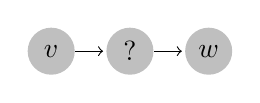
\begin{tikzpicture}[shorten >=1pt,->]
  \tikzstyle{vertex}=[circle,fill=black!25,minimum size=17pt,inner sep=0pt]

  \foreach \name/\x in {v/1, ?/2, w/3}
    \node[vertex] (G-\name) at (\x,0) {$\name$};

  \foreach \from/\to in {v/?, ?/w}
    \draw (G-\from) -- (G-\to);

\end{tikzpicture}}\quad
\subfloat[2-step ($w$ to $v$)]{
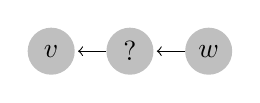
\begin{tikzpicture}[shorten >=1pt,->]
  \tikzstyle{vertex}=[circle,fill=black!25,minimum size=17pt,inner sep=0pt]

  \foreach \name/\x in {v/1, ?/2, w/3}
    \node[vertex] (G-\name) at (\x,0) {$\name$};

  \foreach \from/\to in {w/?, ?/v}
    \draw (G-\from) -- (G-\to);

\end{tikzpicture}}
\\
\subfloat[Mutual (in)]{
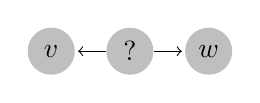
\begin{tikzpicture}[shorten >=1pt,->]
  \tikzstyle{vertex}=[circle,fill=black!25,minimum size=17pt,inner sep=0pt]

  \foreach \name/\x in {v/1, ?/2, w/3}
    \node[vertex] (G-\name) at (\x,0) {$\name$};

  \foreach \from/\to in {?/w, ?/v}
    \draw (G-\from) -- (G-\to);

\end{tikzpicture}}\quad
\subfloat[Mutual (out)]{
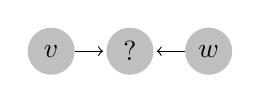
\begin{tikzpicture}[shorten >=1pt,->]
  \tikzstyle{vertex}=[circle,fill=black!25,minimum size=17pt,inner sep=0pt]

  \foreach \name/\x in {v/1, ?/2, w/3}
    \node[vertex] (G-\name) at (\x,0) {$\name$};

  \foreach \from/\to in {w/?, v/?}
    \draw (G-\from) -- (G-\to);

\end{tikzpicture}}
\end{figure}
The importance of ``friends of friends,'' or people two links away from a given node, lends itself to exploring features that directly arise out of the directed @-message graph. 
There are essentially four types of two-step hops, as shown in Figure \ref{fig_2step}, corresponding to either the number of common in-neighbors or out-neighbors (mutual neighbors), or the number of directed paths from $v$ to $w$ or from $w$ to $v$ (two-step paths). 

If both $v$ and $w$ send messages to many common people, it is likely that they are in the same social circle, or that they message the same celebrities. 
If $v$ and $w$ receive many messages from the same group of people, it could be that both $v$ and $w$ are in the same community, or that they are celebrities with overlapping fanbases.

As the number of paths from $v$ to $w$ increases, there are two conflicting forces: $v$ has a stronger source of connections to $w$, but at the same time
$w$ is more popular and hence less likely to reciprocate the $(v,w)$ edge.
The reverse case is simpler--- intuitively, as the number of paths from $w$ to $v$ increases, the likelihood that $w$ will communicate with $v$ grows.

\begin{table}[!t]
\renewcommand{\arraystretch}{1.3}
\caption{Reciprocity Prediction Features}
\label{table_recmethods}
\centering
\begin{tabular}{|c||c|}
\hline
\bf{Feature} & $\mathbf{val}(v)$ or $\mathbf{val}(v,w)$\\
\hline
\multicolumn{2}{|c|}{\emph{Absolute degree/message features}} \\
\hline
Indegree or outdegree & $\deg^-(v)$ or $\deg^+(v)$ \\
Incoming or outgoing messages & $\operatorname{msg}^-(v)$ or $\operatorname{msg}^+(v)$ \\
Message-degree (in or out) & $\frac{\operatorname{msg}^-(v)}{\deg^-(v)}$ or $\frac{\operatorname{msg}^+(v)}{\deg^+(v)}$ \\
Outdegree-indegree & $\frac{\deg^+(v)}{\deg^-(v)}$ \\
\hline
\multicolumn{2}{|c|}{\emph{Relative degree/message features}} \\
\hline
Indegree ratio & $\deg^-(v) / \deg^-(w)$ \\
Outdegree ratio & $\deg^+(v) / \deg^+(w)$ \\
\hline
Incoming message ratio & $\operatorname{msg}^-(v) / \operatorname{msg}^-(w)$ \\
Outgoing message ratio & $\operatorname{msg}^+(v) / \operatorname{msg}^+(w)$ \\
\hline
Message-degree ratio (in) & $\frac{\operatorname{msg}^-(v)}{\deg^-(v)} / \frac{\operatorname{msg}^-(w)}{\deg^-(w)}$ \\
Message-degree ratio (out) & $\frac{\operatorname{msg}^+(v)}{\deg^+(v)} / \frac{\operatorname{msg}^+(w)}{\deg^+(w)}$ \\
\hline
Outdegree-indegree ratio & $\frac{\deg^+(v)}{\deg^-(v)} / \frac{\deg^+(w)}{\deg^-(w)} $ \\
\hline
\multicolumn{2}{|c|}{\emph{Link prediction features}} \\
\hline
Mutual neighbors (in) & $|\Gamma^-(v) \cap \Gamma^-(w)|$ \\
Mutual neighbors (out) & $|\Gamma^+(v) \cap \Gamma^+(w)|$ \\
\hline
Jaccard's coefficient (in) & $\frac{|\Gamma^-(v) \cap \Gamma^-(w)|}{|\Gamma^-(v) \cup \Gamma^-(w)}$ \\
Jaccard's coefficient (out) & $\frac{|\Gamma^+(v) \cap \Gamma^+(w)|}{|\Gamma^+(v) \cup \Gamma^+(w)}$ \\
\hline
Adamic/Adar & $\sum_{\{x|x \in \Gamma^-(v) \cap \Gamma^-(w)\}} \frac{1}{\log{\deg^-(x)}}$ \\
\hline
Preferential attachment ($v$ to $w$) & $\deg^+(v)\cdot \deg^-(w)$ \\
Preferential Attachment ($w$ to $v$) & $\deg^+(w)\cdot \deg^-(v)$ \\
\hline
Two-step paths ($v$ to $w$) & $ |\operatorname{paths}^2(v,w)|$ \\
Two-step paths ($w$ to $v$) & $ |\operatorname{paths}^2(w,v)|$ \\
\hline
Two-step paths ratio & $\frac{|\operatorname{paths}^2(v,w)|}{|\operatorname{paths}^2(w,v)|}$ \\
% $\frac{\sum_{i=1}^2 \beta^i|\operatorname{paths}^i(v,w)|}{\sum_{i=1}^2 \beta^i|\operatorname{paths}^i(w,v)|}$ Did badly
\hline
\end{tabular}
\end{table}

\section{Results and Discussion}

\subsection{Individual properties}
To calculate the accuracy of the individual heuristics, we calculated $\operatorname{val}$ for each feature on the subset $E_{10}^r \cup E_{10}^u$ of the graph $G_{1000}$, where equal numbers of edges were taken from the sets of reciprocated and unreciprocated edges. 
This gives a baseline accuracy is 0.500, achievable by predicting that all edges are of one type. 
We applied the SYM and REV mechanisms to feature sets 2-4, and REV-$v$ and REV-$w$ to set 1.

We then picked a threshold value $\operatorname{val}_{OPT}$ to optimize prediction accuracy - we predicted reciprocity above the threshold, and non-reciprocity below (or vice versa depending on which performed better). 
Tables \ref{table_recresults_indiv} and \ref{table_recresults_indivVW} summarize the performance of each heuristic on the subgraph $G_{1000}, k=10$, while 
table \ref{table_recresults_indeg} summarizes the different mechanisms of prediction for a single heuristic.

In tables \ref{table_recresults_indiv} and \ref{table_recresults_indivVW}, a star ($*$) indicates that reciprocity was predicted when $\operatorname{val}$ was below the threshold, and a lack thereof indicates reciprocity was predicted when $\operatorname{val}$ was above the threshold.

In table \ref{table_recresults_indeg}, SYM$^+$ refers to the prediction mechanism where we aim to predict symmetry and predict all edges with values \emph{above} $val_{OPT}$ to be reciprocated, and REV$^-$ refers to the mechanism where we aim to predict whether a reverse edge $(w,v)$ exists given $(v,w)$ and predict all edges with values \emph{below} $val_{OPT}$ to be reciprocated. 

\subsubsection{Comparison of prediction mechanisms}
We observe higher accuracy for the REV task than SYM, as REV is ``easier" than SYM 
since we know more information about the edge $(v,w)$.

Comparing REV-$v$ to REV-$w$, we see REV-$w$ obtains higher accuracy, suggesting that when trying to predict the existence $(w,v)$ of given $(v,w)$, knowing about properties of $w$ is more valuable than knowing properties of $v$.

Note that SYM$^-$, REV$^-$, REV$-w^+$ and REV-$v^-$ are such poor predictors that simply predicting that everything was reciprocated (or unreciprocated) would have been better.

\subsubsection{Comparison of methods of prediction}

\paragraph{Trends}
On the whole, outdegree-indegree ratio and the two-step paths ratio are the best indicators of reciprocity. 
In fact, outdegree-indegree ratio alone already achieves accuracy to within $\pm 5\%$ of a decision tree using every feature.

\paragraph{Sending and receiving}
When we look at features using one of the four mechanisms, the larger the value, the more likely it is for reciprocation to occur, and this is the case for a majority of features. 
For example, the \emph{larger} the indegree ratio, the more in-links $v$ has in relation to $w$, increasing the probability that $w$ will link to $v$, given that we know that $v$ already links to $w$.

However, the \emph{smaller} the outdegree-indegree ratio, the more likely reciprocation occurs. 
In other words, a large denominator and small numerator in $\frac{\deg^+(v)}{\deg^-(v)} / \frac{\deg^+(w)}{\deg^-(w)} = \frac{\deg^+(v)\deg^-(w)}{\deg^-(v)\deg^+(w)}$ is a good indicator of reciprocation. A large denominator and small numerator indicate that $v$ has many in-links and few out-links and that $w$ has many out-links and few in-links. This suggests that $v$ has higher ``status" than $w$ and hence increases the probability that $w$ links to $v$.

Interestingly, separating the numerator and denominator from the
outdegree-indegree ratio above, which corresponds to our two
preferential attachment features, leads to two very different
results.  While a small numerator does reasonably well (preferential
attachment ($v$ to $w$)), a large denominator does not (preferential
attachment ($w$ to $v$)) and this only performs marginally better than
chance. It is reasonable that the numerator and denotimatior
individially perform worse than the ratio, since the ratio takes into
account both of them. However, the fact that the denominator performs
so poorly is very surprising because a large denominator suggests
that $v$ has a higher status than $w$, and it also causes a higher
chance that $w$ links to $v$ even if $w$ were to pick who to link to
at random. On the other hand, a small numerator makes a statement
about status but not about higher chances of reciprocation under a
random process. The fact that a small numerator is more important than
a large denominator suggests that status (measured by the number of in
and out links) is a very powerful predictor for reciprocity.

If we only consider edges $E_= = \{(v,w)~|~\deg^-(v) = \deg^-(w)\}$, or that both nodes in every node pair have equal indegree, the accuracy of the outdegree ratio feature rises to 0.811. This result is comparable to what we get for the outdegree-indegree ratio feature, which is unsurprising as that reduces to outdegree ratio with equal indegree. 

\paragraph{REV-$v$ vs. REV-$w$}
Not surprisingly, REV-$w$ performs better than REV-$v$ on almost all features, and where REV-$v$ performs better, 
the difference is not as significant.
The fact that information about $w$ is more useful than information
about $v$ forms a suggestive contrast for various domains of
potential application: for example, if we think of $v$ as sending 
information to $w$ via the $(v,w)$ communication link (consider for example
a marketer $v$ contacting a potential customer $w$), then we find
that knowledge of the recipient ($w$) tells us more about the 
probability of a response than knowledge of the sender ($v$).

\begin{table}[!t]
\renewcommand{\arraystretch}{1.3}
\caption{Indegree performance - different methods}
\label{table_recresults_indeg}
\centering
\begin{tabular}{|c||c|c|}
\hline
\bf{Mechanism} & $\mathbf{val}_{OPT}$ (Percentile) & \bf{Accuracy} \\
\hline
\multicolumn{3}{|c|}{\emph{Indegree ratio}} \\
\hline
SYM$^+$ & 0.256 (40) & 0.702 \\
SYM$^-$ & - & - \\
REV$^+$ & 0.414 (46) & 0.759 \\
REV$^-$ & - & - \\
\hline
\multicolumn{3}{|c|}{\emph{Indegree of $v$ or $w$}} \\
\hline
REV-$w^+$ & - & - \\
REV-$w^-$ & 74 (61) & 0.731 \\
REV-$v^+$ &  61 (60) & 0.582 \\
REV-$v^-$ & - & - \\
\hline
\end{tabular}
\end{table}

\begin{table}[!t]
\renewcommand{\arraystretch}{1.3}
\caption{Reciprocity Prediction Method Performance: Individual (REV)}
\label{table_recresults_indiv}
\centering
\begin{tabular}{|c||c|c|}
\hline
\bf{Method} & $\mathbf{val}_{OPT}$ (Percentile) & \bf{Accuracy} \\
\hline
Indegree ratio & 0.414 (46) & 0.759 \\
Outdegree ratio & 0.667 (43) & 0.628 \\
\hline
Incoming message ratio & 0.333 (48) & 0.772 \\
Outgoing message ratio & 0.905 (46) & 0.547 \\
\hline
Incoming message-indegree ratio & 0.650 (39) & 0.569 \\
Outgoing message-outdegree ratio & 0.791 (33) & 0.615* \\
\hline
Outdegree-indegree ratio & 1.72 (53) & 0.820* \\
\hline
Mutual neighbors (in) & 10 (61) & 0.552 \\
Mutual neighbors (out) & 8 (51) & 0.580 \\
\hline
Jaccard's coefficient (in) & 0.0345 (48) & 0.684 \\
Jaccard's coefficient (out) & 0.0637 (55) & 0.660 \\
\hline
Adamic/Adar & 1.94 (55) & 0.561 \\
\hline
Two-step paths ($v$ to $w$) & 6 (59) & 0.517* \\
Two-step paths ($w$ to $v$) & 5 (51) & 0.657 \\
Two-step paths ratio & 0.556 (52) & 0.760 \\
% Two-step paths ratio (undirected) & 0.259 (34) & 0.516 \\
\hline
Preferential attachment ($v$ to $w$) & 10230 (58) & 0.687* \\
Preferential attachment ($w$ to $v$) & 2610 (37) & 0.534* \\
\hline
\end{tabular}
\end{table}

\begin{table}[!t]
\renewcommand{\arraystretch}{1.3}
\caption{Reciprocity Prediction Method Performance: Individual (REV-$v$,REV-$w$)}
\label{table_recresults_indivVW}
\centering
\begin{tabular}{|c||c|c|}
\hline
\bf{Method} & $\mathbf{val}_{OPT}$ (Percentile) & \bf{Accuracy} \\
\hline
Indegree (v) &  61 (60) & 0.582 \\
Indegree (w) & 148 (61) & 0.731* \\
Outdegree (v) & 25 (14) & 0.506* \\
Outdegree (w) & 105 (60) & 0.647* \\
\hline
Incoming messages (v) & 619 (53) & 0.637 \\
Incoming messages (w) & 1802 (54) & 0.733* \\
Outgoing messages (v) & 906 (51) & 0.542 \\
Outgoing messages (w) & 506 (17) & 0.524* \\
\hline
Incoming message-indegree (v) & 9.4 (41) & 0.596 \\
Incoming message-indegree (w) & 9.12 (30) & 0.535 \\
Outgoing message-outdegree (v) & 13.2 (50) & 0.523 \\
Outgoing message-outdegree (w) & 8.14 (36) & 0.661 \\
\hline
Outdegree-indegree (v) & 1.28 (53) & 0.679* \\
Outdegree-indegree (w) & 0.747 (50) & 0.777 \\
\hline
\end{tabular}
\end{table}

\subsection{Decision tree analysis}

We then combined subsets of features and evaluated their performance by splitting the edges in $E^r_{10} \cup E_{10}^u$ randomly into two sets and performing 2-fold cross-validation. The ID3 algorithm was used, and because $\operatorname{val}$ is continuous, we split each into deciles (dividing the data equally into tenths) to reduce computation time.

The following combined subsets, in addition to each individual subset, were considered:
\begin{enumerate}
	\item {\bf All} (sets 1-4) -- every single feature was considered.
	\item {\bf All ratio} (sets 2,3,4) -- all features that used ratios were considered.
	\item {\bf All absolute} (sets 1,3,4) -- we wanted to see how using ``absolute'' features would affect our decision accuracy.
\end{enumerate}
\begin{table}[!t]
\renewcommand{\arraystretch}{1.3}
\caption{Decision Tree Accuracy}
\label{table_recresults_dtree}
\centering
\begin{tabular}{|c||c|c|}
\hline
\bf{Set} & Accuracy & Top-level attribute \\
\hline
Degree/message (1) & 0.832 & Outdegree-indegree (w) \\
Degree/message ratio (2) & 0.861 & Outdegree-indegree ratio \\
Two-step hops (3) & 0.796 & Two-step paths ($w$ to $v$) \\
Link prediction (4) & 0.739 & Two-step paths ratio (directed) \\
\hline
\multicolumn{3}{|c|}{\emph{Combined}} \\
\hline
All ratio (2,3,4) & 0.861 & Outdegree-indegree ratio \\
All absolute (1,3,4) & 0.832 & Outdegree-indegree (w) \\
All (1-4) & 0.862 & Outdegree-indegree ratio \\
\hline
\end{tabular}
\end{table}

Table \ref{table_recresults_dtree} shows the accuracy of the trees and
their most important attribute for the different sets of features. We
find that the accuracy when we only use degree/message features
compared to that when we include all features is the same. And
although we observe that the two-step paths ratio obtains an accuracy
of 0.760 on its own while the decision tree for link prediction only
manages 0.739, this can be attributed to the inaccuracy introduced
splitting each continuous variable into 10 discrete portions.
Furthemore, features commonly used for
link prediction yield a tree of lower accuracy than other features, establishing a concrete sense in which 
the problem of reciprocity prediction is different
from link prediction.

Whenever the outdegree-indegree value or ratio was included as an attribute, it became the most important.

If we only consider $E_=$, node pairs with equal indegree ($|E_=|=16,311$), the accuracy of All ratio drops to 0.776, suggesting that predicting reciprocity here is considerably more difficult as we lose the ability to differentiate nodes of different status, or indegree. 
Again, the most important feature is outdegree ratio.

\subsection{Regression analysis}
We also used a logistic regression model on subsets of features as well, where $f(z) = \frac{e^z}{e^z+1}$, $z = \beta_0 + \beta F$, $f(z)$ is binary (1 when an edge is reciprocated, 0 otherwise) and $F$ is the vector of features.
The results are shown in tables \ref{table_recresults_logr}---\ref{table_recresults_lograll3}, where struck-out $\mathbf{p}$-values indicate insignificant features. 
Here, we see that the two-step paths ($v$ to $w$), the two-step paths ratio and Jaccard (out) features are most significant even when taking into account all features at once.


\begin{table}[!t]
\renewcommand{\arraystretch}{1.3}
\caption{Logistic regression -- relative degree/message-based features}
\label{table_recresults_logr}
\centering
\begin{tabular}{|c||c|c|}
\hline
\bf{Feature} & $\mathbf{\beta}$ & $\mathbf{p}$ value \\
\hline
Indegree ratio & 0.0101903 & $< 2 \e{-16} $ \\
Outdegree ratio & 0.0005775 & \sout{0.2545} \\
Incoming messages ratio & 0.0230161 & $< 2 \e{-16} $ \\
Outgoing messages ratio & -0.0047152 & $< 2 \e{-16} $ \\
Incoming messages-indegree ratio & -0.0005545 & \sout{0.0798} \\
Outgoing messages-outdegree ratio & -0.0049387 & $< 2 \e{-16} $ \\
Outdegree-indegree ratio & \bf{-0.0562983} & $< 2 \e{-16} $ \\
\hline
\end{tabular}
\end{table}

\begin{table}[!t]
\renewcommand{\arraystretch}{1.3}
\caption{Logistic regression -- two-step hop features}
\label{table_recresults_logrpath}
\centering
\begin{tabular}{|c||c|c|}
\hline
\bf{Feature} & $\mathbf{\beta}$ & $\mathbf{p}$ value \\
\hline
Mutual neighbors (in) & -0.0117269 & $< 2 \e{-16} $ \\
Mutual neighbors (out) & 0.0180579 & $< 2 \e{-16} $ \\
Two-step paths ($v$ to $w$) & -0.1193624 & $< 2 \e{-16} $ \\
Two-step paths ($w$ to $v$) & 0.1296081 & $< 2 \e{-16} $ \\
\hline
\end{tabular}
\end{table}

\begin{table}[!t]
\renewcommand{\arraystretch}{1.3}
\caption{Logistic regression -- All ratio}
\label{table_recresults_lograll2}
\centering
\begin{tabular}{|c||c|c|}
\hline
\bf{Feature} & $\mathbf{\beta}$ & $\mathbf{p}$ value \\
\hline
Indegree ratio     &    0.0120256  & $< 2 \e{-16} $\\
Outdegree ratio    &   -0.0015554  & 0.005739 \\
Incoming messages ratio    &    0.0145437  & $< 2 \e{-16} $\\
Outgoing messages ratio   &   -0.0043189  & $< 2 \e{-16} $\\
Incoming messages-indegree ratio   & 0.0048525   & $< 2 \e{-16} $ \\
Outgoing messages-outdegree ratio   & -0.0046674 & $< 2 \e{-16} $ \\
Outdegree-indegree ratio  &  -0.0301592  & $< 2 \e{-16} $\\
\hline
Mutual Neighbors (in) & -0.0279290  &$< 2 \e{-16} $\\
Mutual Neighbors (out) & 0.0147103  & $< 2 \e{-16} $\\
Two-step paths ($v$ to $w$)  &  \bf{-0.0530463}   & $< 2 \e{-16} $\\
Two-step paths ($w$ to $v$)   &    0.0182572   & $< 2 \e{-16} $\\
\hline
Two-step paths ratio  &   \bf{0.0394657} & $< 2 \e{-16} $\\
Jaccard (in) & -0.0238541 & $< 2 \e{-16} $\\
Jaccard (out) &   \bf{0.0572358}  & $< 2 \e{-16} $\\
Adamic-Adar  &    -0.0001424 & \sout{0.881637} \\
Preferential attachment ($v$ to $w$) & 0.0010837  & 0.000627 \\
Preferential attachment ($w$ to $v$)  &  - & -  \\
\hline
\end{tabular}
\end{table}

\begin{table}[!t]
\renewcommand{\arraystretch}{1.3}
\caption{Logistic regression - All}
\label{table_recresults_lograll3}
\centering
\begin{tabular}{|c||c|c|}
\hline
\bf{Feature} & $\mathbf{\beta}$ & $\mathbf{p}$ value \\
\hline
Indegree ratio     &    0.0041791  & $6.09\e{-8}$  \\
Outdegree ratio    & 0.0046914 & $1.28\e{-13}$ \\
Incoming messages ratio    &   0.0029794  & 0.000125 \\
Outgoing messages ratio   &   0.0033361  & $3.10\e{-10}$ \\
Incoming messages-indegree ratio & 0.0040884 &  $1.11\e{-14}$ \\
Outgoing messages-outdegree ratio &  -0.0015075 &  0.006283 \\
Outdegree-indegree ratio  &   -0.0057958 & $< 2 \e{-16} $\\
\hline
Indegree (v) & 0.0050520 & $ 4.30 \e{-11}$ \\
Indegree (w) & -0.0089197 & $<2 \e{-16} $ \\
Outdegree (v) & -0.0063247 & $<2 \e{-16}$ \\
Outdegree (w) & 0.0035881 & $3.58\e{-7}$ \\
Incoming messages (v) & 0.0063390 & $<2 \e{-16} $ \\
Incoming messages (w) & -0.0179975 & $<2 \e{-16} $ \\
Outgoing messages (v) & -0.0070869 & $<2 \e{-16} $\\
Outgoing messages (w) & 0.0095572 & $<2 \e{-16} $ \\
Incoming message-indegree (v) & -0.0023250 & $1.11\e{-5}$ \\
Incoming message-indegree (w) & -0.0004044 & \sout{0.42781} \\
Outgoing message-outdegree (v) & 0.0007430 & \sout{0.175454}  \\
Outgoing message-outdegree (w) & 0.0024155 & $2.54\e{-5}$ \\
Outdegree-indegree (v) & -0.0110324 & $<2 \e{-16} $ \\
Outdegree-indegree (w) & 0.0218874 & $<2 \e{-16} $ \\
\hline
Mutual Neighbors (in) &-0.0194635  &$< 2 \e{-16} $\\
Mutual Neighbors (out) &0.0050245  & $< 2 \e{-16} $\\
Two-step paths ($v$ to $w$)  &  -0.0462950   & $< 2 \e{-16} $\\
Two-step paths ($w$ to $v$)   &    0.0167156  & $< 2 \e{-16} $\\
\hline
Two-step paths ratio &   0.0440107 & $< 2 \e{-16} $\\
Jaccard (in) & -0.0398243 & $< 2 \e{-16} $\\
Jaccard (out) &   0.0561815  & $< 2 \e{-16} $\\
Adamic-Adar  & 0.0111504 & $< 2 \e{-16} $ \\
Preferential attachment ($v$ to $w$) & 0.0009537 & 0.003002 \\
Preferential attachment ($w$ to $v$)  &  - & -  \\
\hline
\end{tabular}
\end{table}

\section{Twitter as a superposition of networks}

\subsection{(Un)reciprocated subgraph analysis}
We also analyze how various properties of the subgraphs $G_n$, as well as the edge sets $E^r_k$ and $E^u_k$ vary as we adjust $n$ and $k$.

\paragraph*{Reciprocated and unreciprocated edges} We observe that the frequency of reciprocated edges is approximately 2 to 3 times that of unreciprocated edges, and the proportion of reciprocated edges increases as $n$ and $k$ increases (Fig. \ref{fig_rur_propn}, \ref{fig_rur_propk}). 
While reciprocated communication is the dominant form of interaction, we see a significant number of ``unreciprocated'' interaction, indicating that a significant number of relationships on Twitter are unbalanced. 
This could occur when a user of lower status repeatedly invokes
the name of a
more influential user (of higher status) through messaging,
as suggested in the introduction.

\paragraph*{Reciprocated and unreciprocated nodes} A majority of nodes have reciprocated relationships, with a small proportion having only unreciprocated relationships. 
A significant proportion of nodes take part in both reciprocated and unreciprocated relationships - indicating that while there are two distinct types of relationships occurring on Twitter, this does not correspond to two distinct types of users. 
The fact that it is rare to find 
active Twitter users taking part in only unreciprocated interactions
suggests a sense in which 
social (reciprocated) relationships may be the 
driving force in the active and continued use of the platform.

We can also see this in Fig. \ref{fig_rur_sca2}, a scatter plot of the
number of users $v$ with each of three types of interaction:
(i) reciprocal relationships with both $(v,w)$ and $(w,v)$ present;
(ii) unreciprocated ``out-going'' relationships with only $(v,w)$ present;
and 
(iii) unreciprocated ``in-coming'' relationships with only $(w,v)$ present.
We thus differentiate between both ends in an
unreciprocated edge ($v \xrightarrow{k} w$ and $w \xrightarrow{=0} v$),
where a user could be $v$ if she's not replied to, or $w$ if she
doesn't reply.  The most common type of nodes are those which only
have reciprocated edges, with far fewer having unreciprocated
interactions of some type.

\paragraph*{Clustering coefficient remains relatively stable as $n$, $k$ vary}
The clustering coefficient is much larger in the subgraph of reciprocated
edges, which corresponds naturally to the notion that reciprocated 
edges represent more social activity, with a larger density of triangles.
The fact that these quantities are stable as we change $n$ and $k$ suggests
that the network properties of these subgraphs do not change significantly even if we sample from a relatively smaller population of all users (Fig. \ref{fig_rur_cc_n},\ref{fig_rur_cc_k}).

\paragraph*{Connected component remains stable as $n$ varies, but decreases as $k$ increases} 
The graphs corresponding to $E_k^r$ and $E_k^u$ have giant components
for relatively low values of $k$.
However, the size of the largest component shrinks rapidly once 
$k$ passes a particular range (roughly between 50 and 100).
(Fig. \ref{fig_rur_lcc_n},\ref{fig_rur_lcc_k}).
This hints at a kind of qualitative transition in the structure of the
network as a function of message volume, with the edges representing 
more than 100 communications each being unable to sustain a very large
component on their own.

\begin{figure}[!t]
\centering
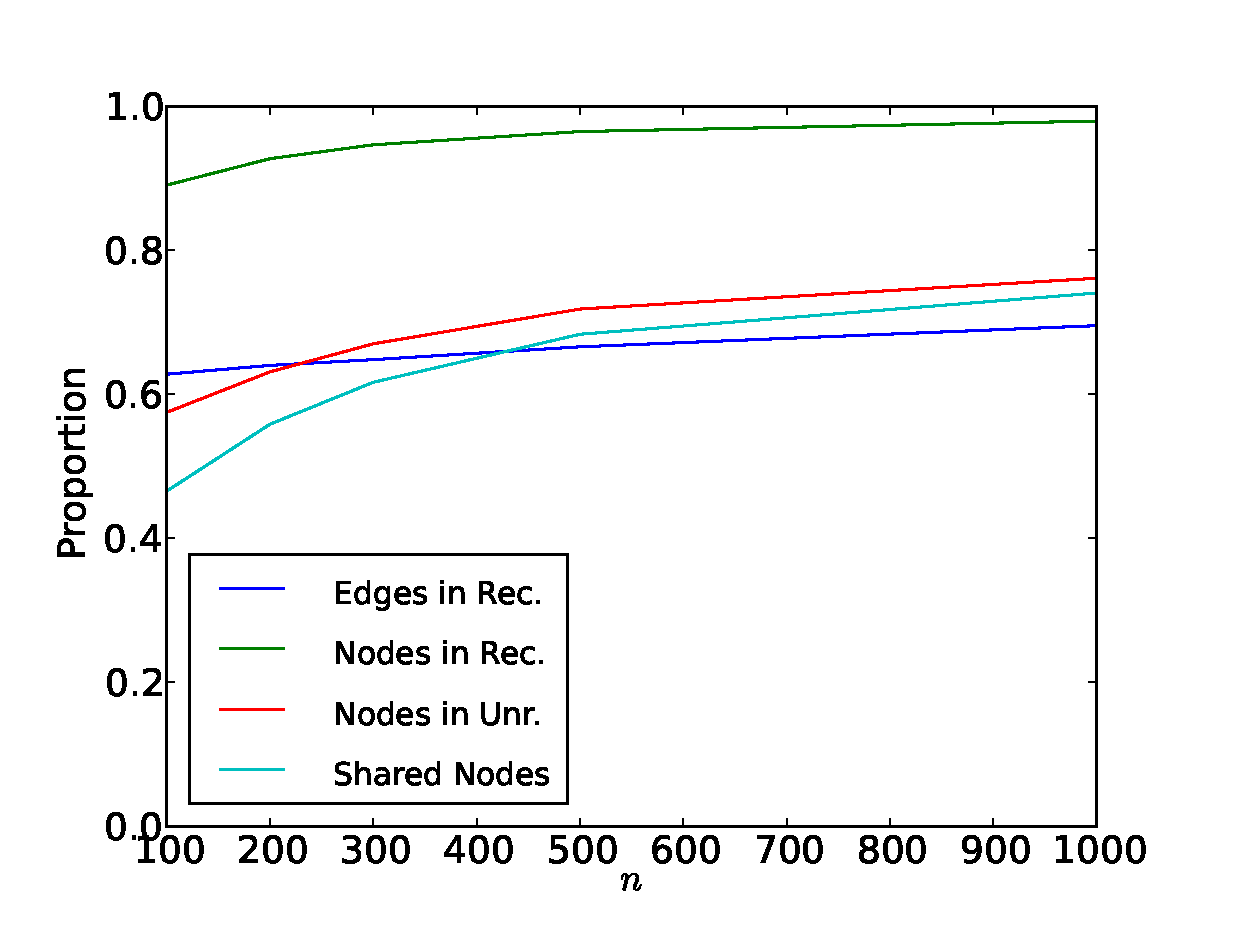
\includegraphics[width=2.5in]{proportion_edgesnodes_n}                
\caption{Proportion of nodes or edges (varying $n$)}
\label{fig_rur_propn}
\end{figure}

\begin{figure}[!t]
\centering
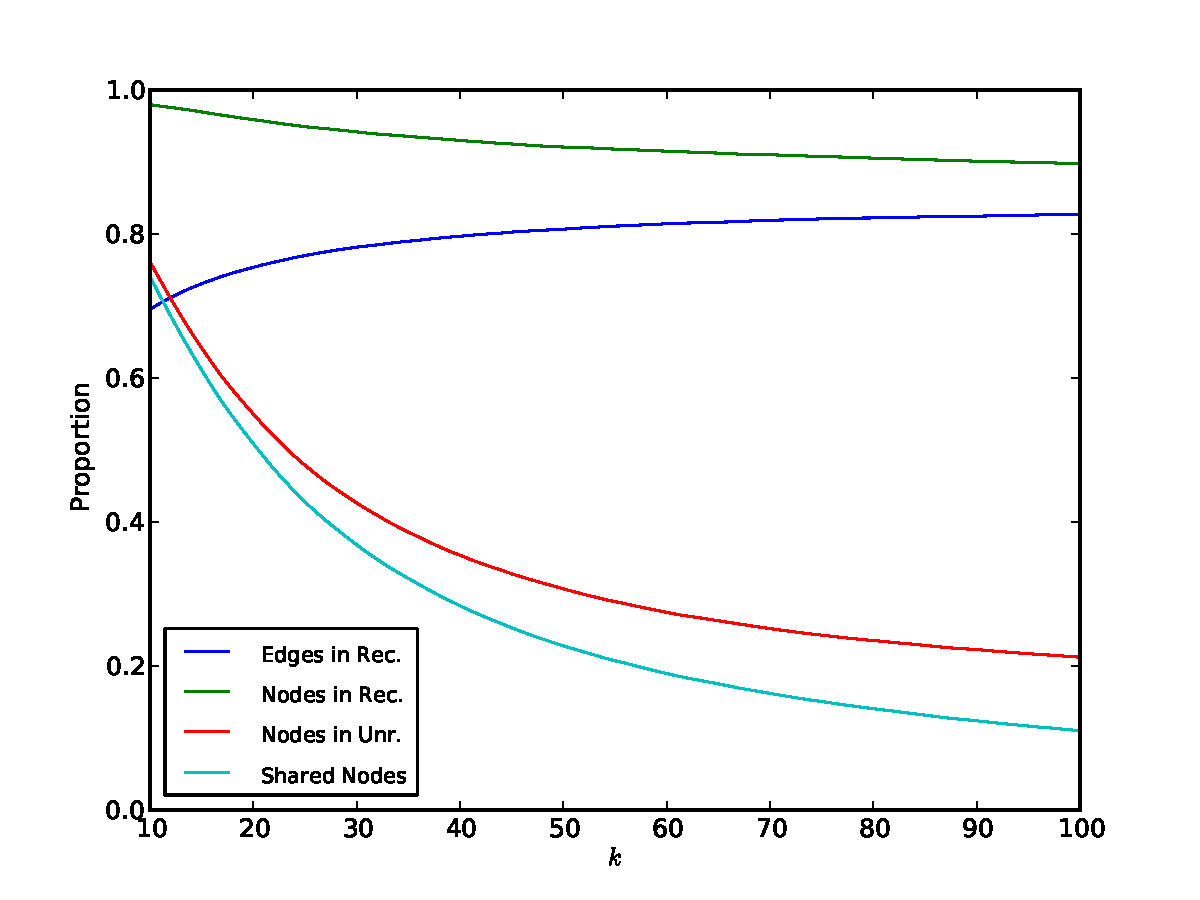
\includegraphics[width=2.5in]{proportion_edgesnodes_k}                
\caption{Proportion of nodes or edges (varying $k$)}
\label{fig_rur_propk}
\end{figure}

\begin{figure}[!t]
\centering
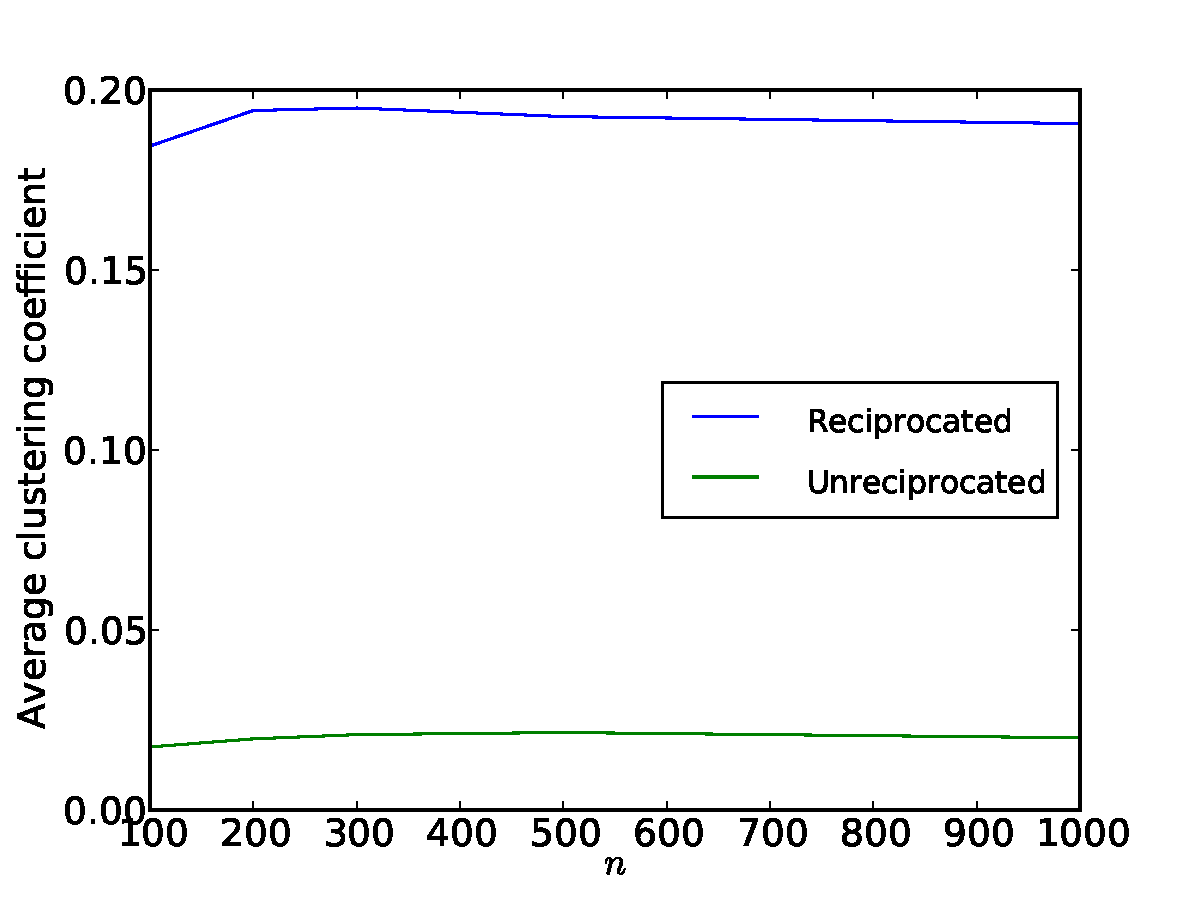
\includegraphics[width=2.5in]{average_clustering_n}          
\caption{Clustering coefficient (varying $n$)}
\label{fig_rur_cc_n}
\end{figure}

\begin{figure}[!t]
\centering
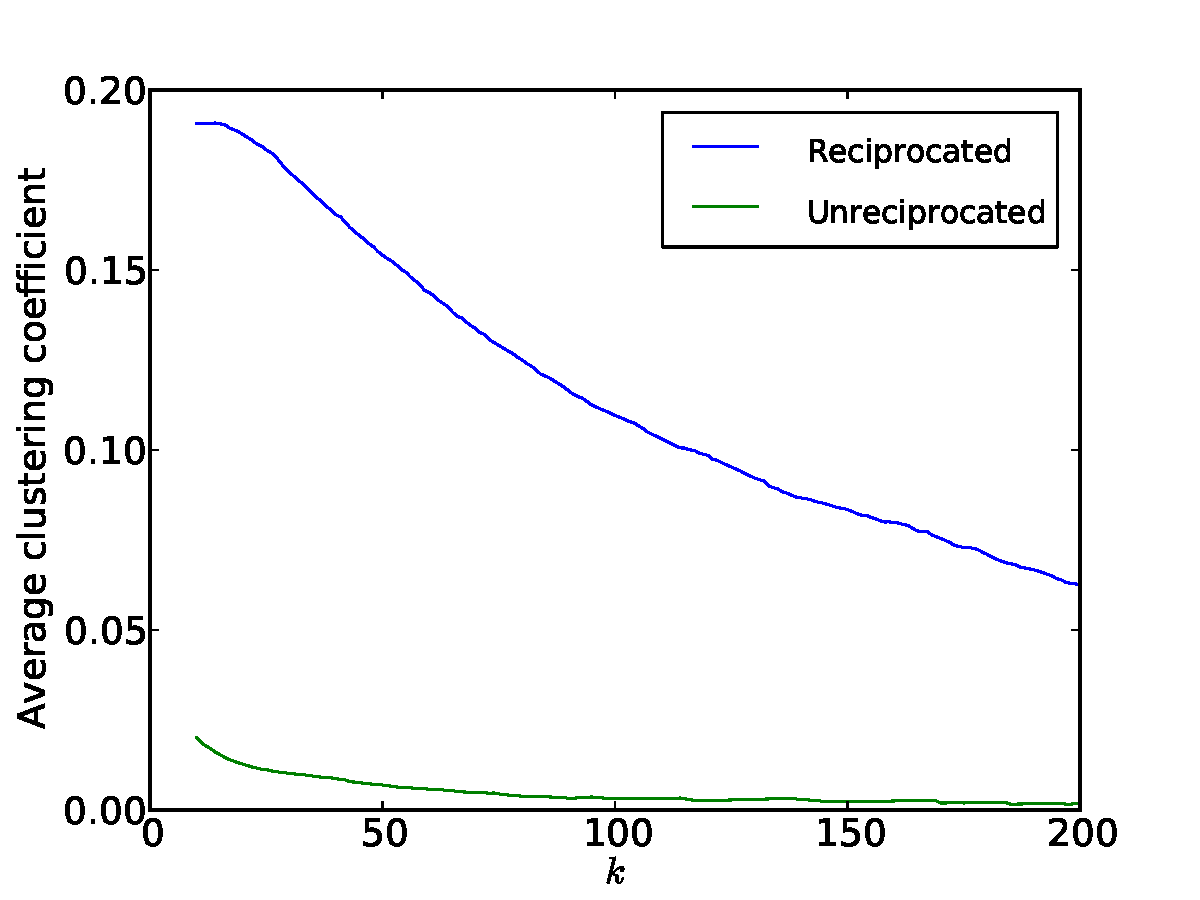
\includegraphics[width=2.5in]{average_clustering_k}      
\caption{Clustering coefficient (varying $k$)}
\label{fig_rur_cc_k}
\end{figure}

\begin{figure}[!t]
\centering
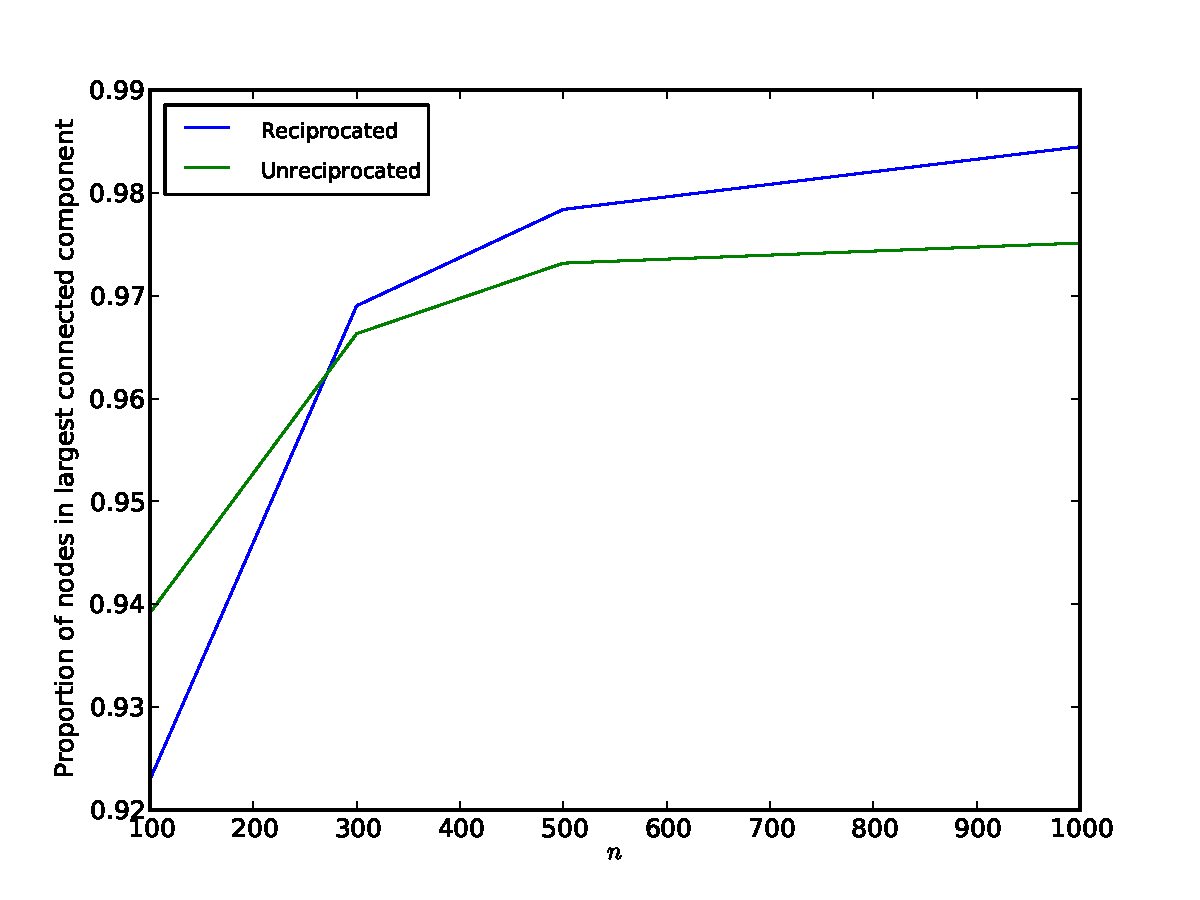
\includegraphics[width=2.5in]{proportion_largestcc_n}
\caption{Proportion in largest connected component (varying $n$)}
\label{fig_rur_lcc_n}
\end{figure}

\begin{figure}[!t]
\centering
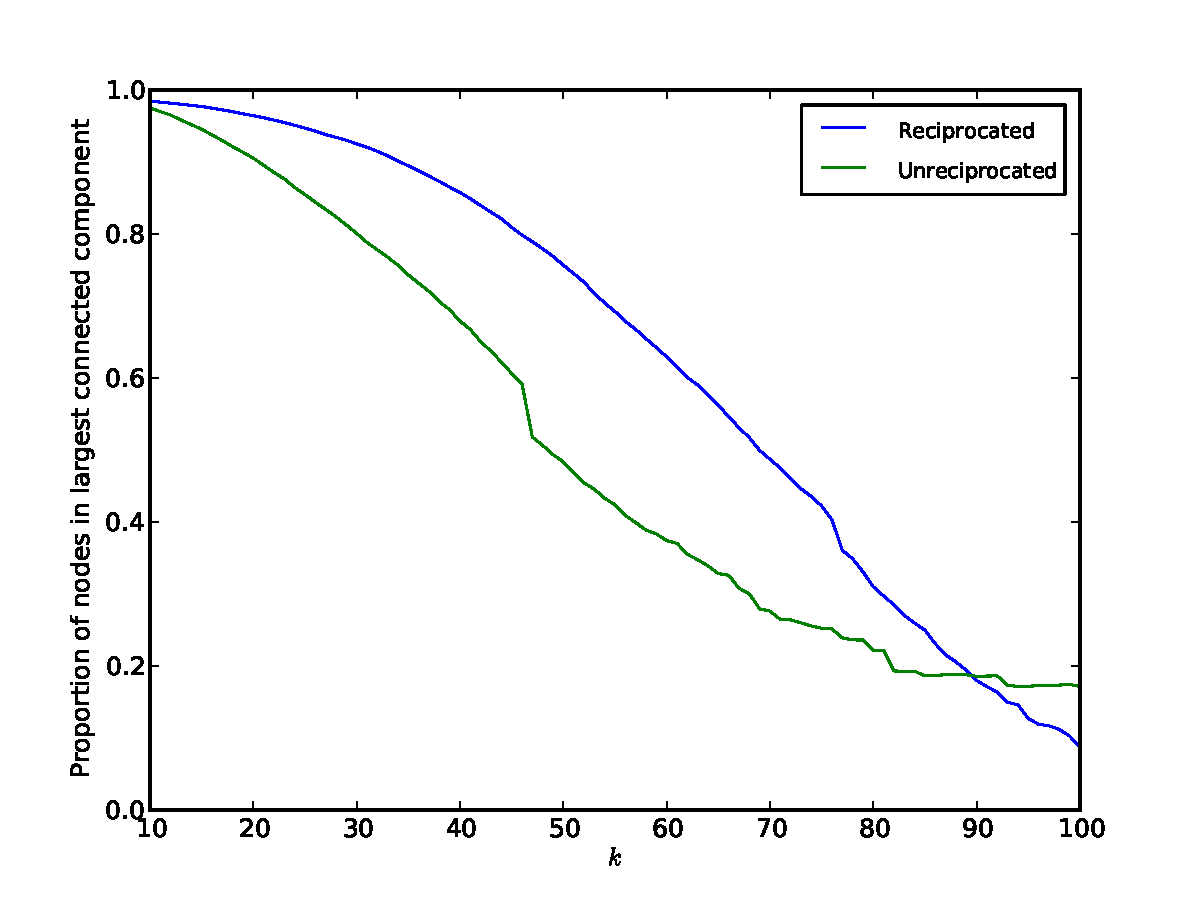
\includegraphics[width=2.5in]{proportion_largestcc_k}
\caption{Proportion in largest connected component (varying $k$)}
\label{fig_rur_lcc_k}
\end{figure}

%\begin{figure}[!t]
%\centering
%\subfloat[Varying $n$]{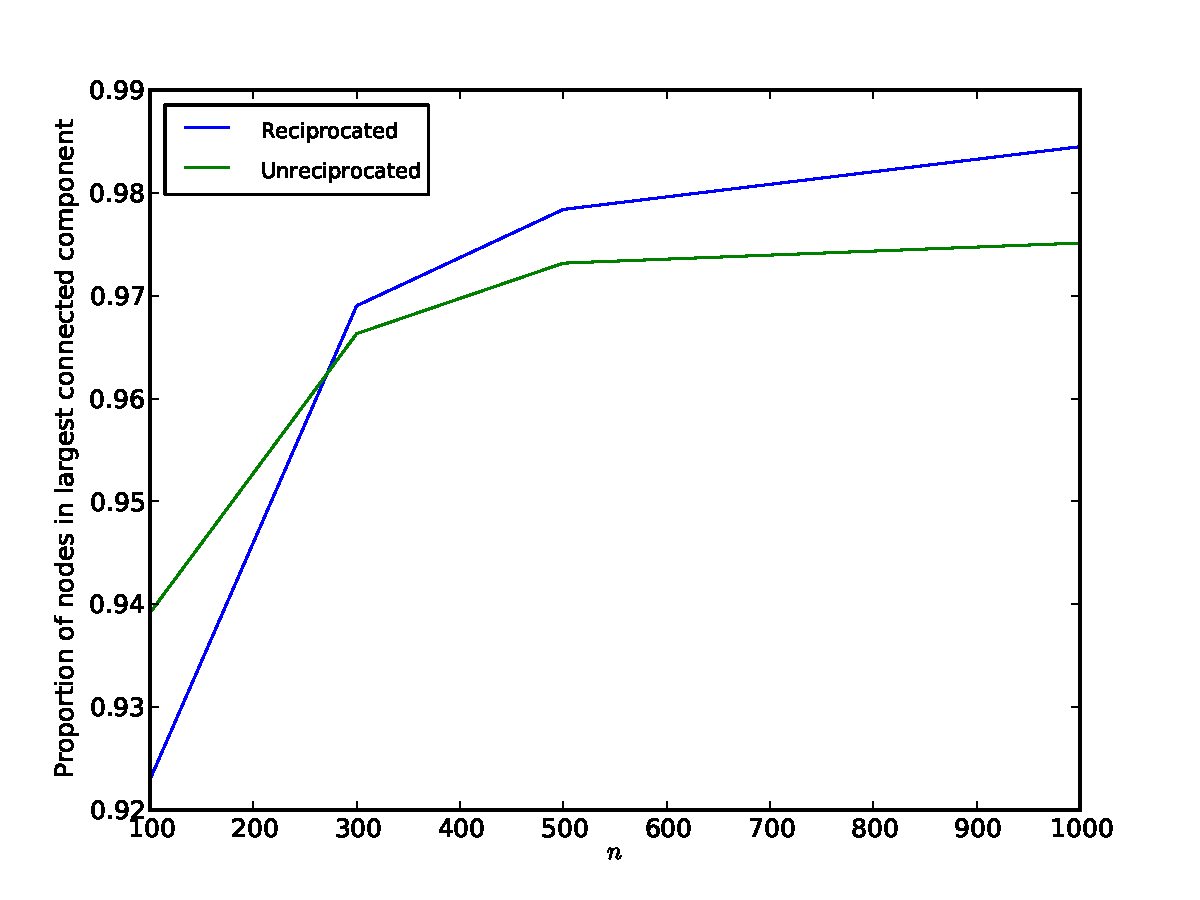
\includegraphics[width=1.5in]{proportion_largestcc_n}}                
%\subfloat[Varying $k$]{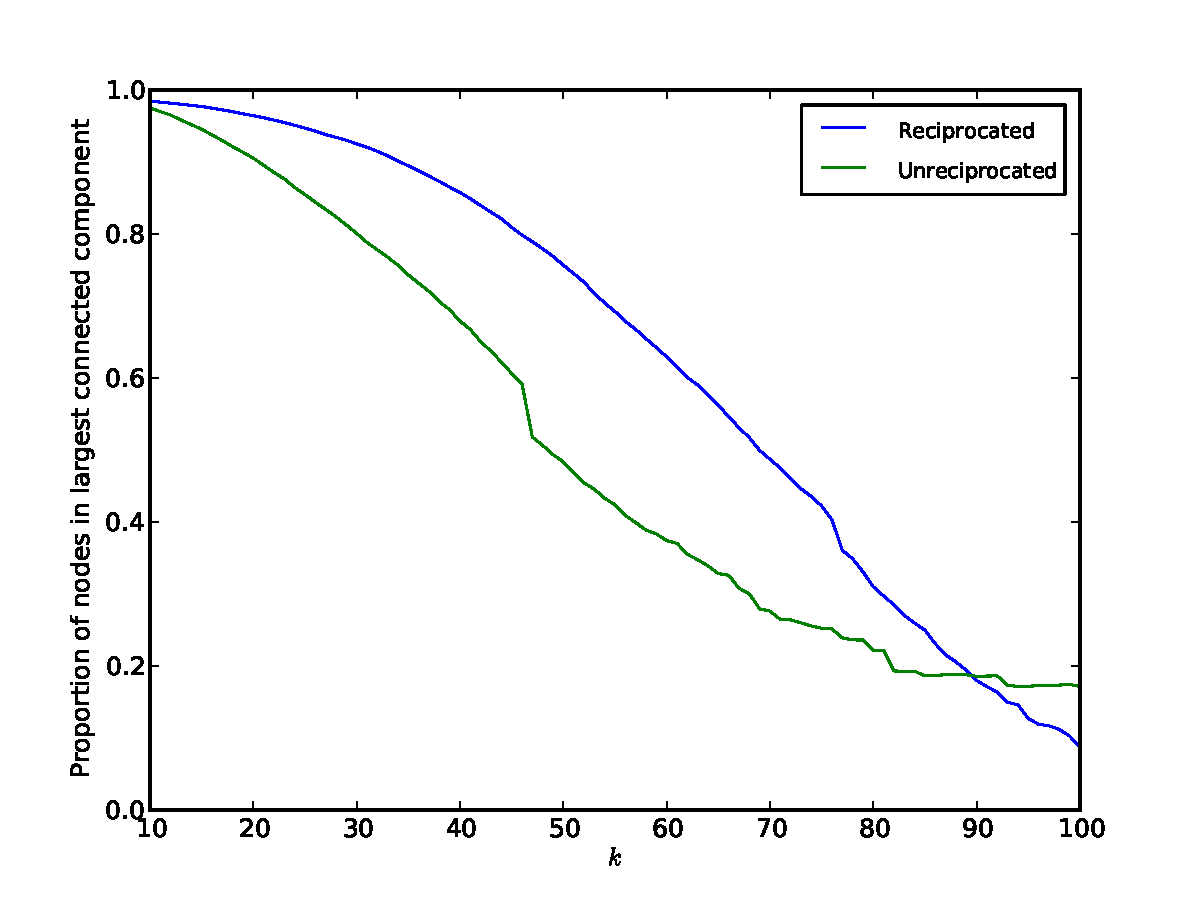
\includegraphics[width=1.5in]{proportion_largestcc_k}}
%\caption{Proportion in largest connected component}
%\label{fig_rur_lcc}
%\end{figure}

\begin{figure}[!t]
\centering
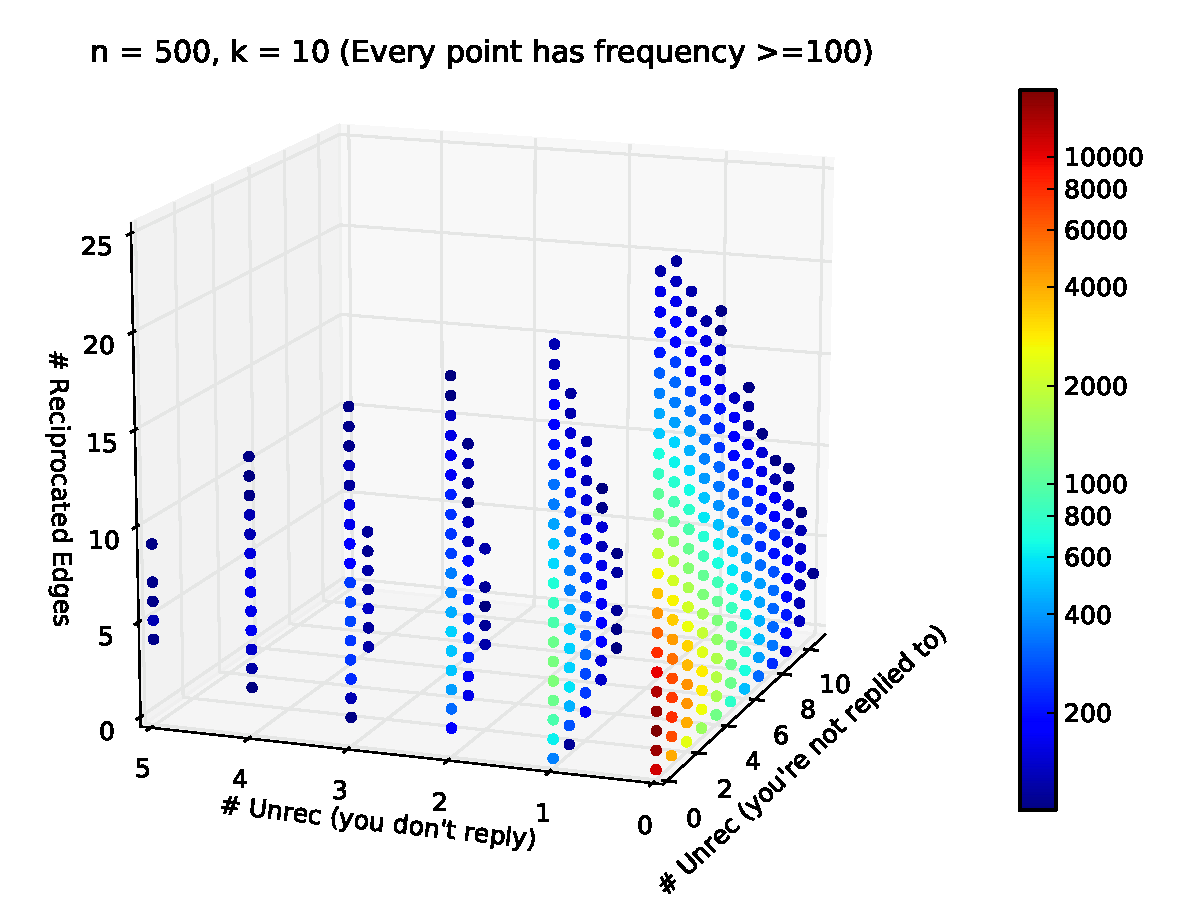
\includegraphics[width=2.5in]{scatter3}
\caption{Scatter plot of users' interaction types}
\label{fig_rur_sca2}
\end{figure}

% An example of a double column floating figure using two subfigures.
% (The subfig.sty package must be loaded for this to work.)
% The subfigure \label commands are set within each subfloat command, the
% \label for the overall figure must come after \caption.
% \hfil must be used as a separator to get equal spacing.
% The subfigure.sty package works much the same way, except \subfigure is
% used instead of \subfloat.
%
%\begin{figure*}[!t]
%\centerline{\subfloat[Case I]\includegraphics[width=2.5in]{subfigcase1}%
%\label{fig_first_case}}
%\hfil
%\subfloat[Case II]{\includegraphics[width=2.5in]{subfigcase2}%
%\label{fig_second_case}}}
%\caption{Simulation results}
%\label{fig_sim}
%\end{figure*}
%
% Note that often IEEE papers with subfigures do not employ subfigure
% captions (using the optional argument to \subfloat), but instead will
% reference/describe all of them (a), (b), etc., within the main caption.

\section{Conclusion}

We have formulated several variants of the problem of 
reciprocity prediction in an on-line social network, and we
have obtained strong performance
using properties of nodes and their local network neighborhoods.
In particular, features that approximate the relative status of
two nodes $v$ and $w$ appear to be the most effective at 
predicting whether a link between $v$ and $w$ will be reciprocal.
We have also studied the subgraphs of reciprocated and unreciprocated
links, finding that they differ in important ways with respect
to component sizes and clustering.

There are a number of interesting further directions that could
pursued on this problem.
First, our approach has used structural features of the system,
but it would be very interesting to combine these with other
data such as textual content to obtain
stronger estimates of reciprocation.
Second, temporal information is another important source of data
in analyzing reciprocation, and understanding how reciprocated
and unreciprocated interactions develop over time could provide
further insight into the problem.
And third, we should remember that reciprocation is one aspect of
the broader issue of heterogeneity in the types of interactions
encountered on a site such as Twitter, and finding other
dimensions along which to express this heterogeneity is an 
important question as well.


% \section*{Acknowledgment}
 % This work was supported by (SOMEGRANT).


\bibliographystyle{IEEEtran}
\bibliography{rec}

\end{document}


